\documentclass[12pt,a4paper]{moderncv}
\usepackage{color}
\usepackage{graphicx}

\moderncvtheme[green]{classic}

\firstname{Peter}
%\firstname{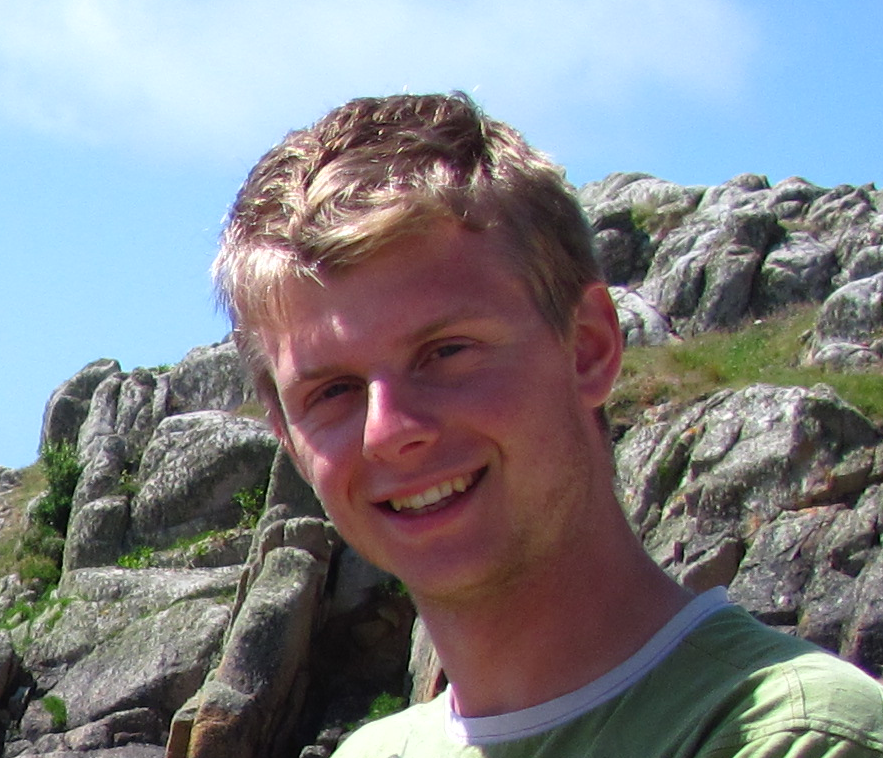
\includegraphics[width=0.3\linewidth]{face} Peter}
\familyname{Saxton}


\address{Flat 7, Wavel Court}{E1W 3QT, London}
%\phone{+44 (0)1884~266~249}
%\mobile{+44 (0)7596~279~256}
\email{peter.saxton@worc.oxon.org}
%\quote{wee}

%\photo[64pt][0.4pt]{face}

\begin{document}
\maketitle

\section{Education}
\cventry{2011--2012}{Research}{Heriot Watt University}{Edinburgh}{}
{Project title: Waveguide Integrated Superconducting Nanowire Single Photon Detectors}

\cventry{2006--2010}{Physics MPhys}{Oxford University}{Oxford}{\textit{1st Class}}{Final year courses: Atmospheres and Oceans, Condensed Matter Physics}

\cventry{1999--2006}{Colyton Grammar School}{Devon}{}{}{
\begin{description}
\item[A-levels:] Mathematics [A], Chemistry [A], Physics [A], Further Maths [A]
\item[Advanced Extension Award:] Mathematics [Merit], Chemistry [Distinction]
\item[GCSEs] Mathematics [A*], Physics [A*], Chemistry [A*], Geography [A*], Biology [A], Religious education [A], English Literature [A], German [A], French [B], English [B], Design and Technology [B]
\end{description}}

\section{Employment}
\cventry{2011--2011}{Software Developer}{Siemens Magnet Technology}{Enysham}{Oxon}{I was placed with the magnet team for the development of a high speed data logger. This system was to monitor up to 40 channels at microsecond resolution. My role was to devise and program algorithms to filter for events on the magnet, saving these and automatically discarding the rest of the raw data. Through this project I became competent with LabView.}

\cventry{2010}{Delivery driver}{Majestic Wines}{Blackwall}{London}{Responsibilities including packing, checking orders as well as route planning.}

\cventry{2010}{Temporary work}{Manpower}{Exeter}{Devon}{I was employed in a number of roles including cleaning at a quarry, assisting a professional photographer and working nights in a Royal Mail sorting office.}

\cventry{2008}{Summer Placement}{Siemens Magnet Technology}{Enysham}{Oxon}{I was given an independent project to design, build and test an experimental persistent current switch with the aim of investigating current distributions in multi-strand wire. This project taught me a variety of practical skills as well as useful experience working with several people across a large organisation.}

\cventry{2007}{Summer Work}{South West Event Hire}{Exeter}{Devon}{I worked in a warehouse preparing orders for delivery and sorting stock when it was returned. This required meticulous attention to detail as well as meeting tight deadlines.}

\section{Additional Information}
\subsection{Practical skills}
\cvitem{Experimental}{I have worked cryogenics, vacuum systems, microwave electronics and high current applications. I have also received training for the safe handling of gas cylinders.}
\cvitem{Driving Licence}{Clean Driving licence for 7 years}
\subsection{Computer Skills}
\cvitem{\emph{Python}}{This is the main language I have used in the last 12 months. Nearly every experiment run has required new code to be written. I have also been working to create well documented standard libraries for our equipment to save time in future development.}
\cvitem{\emph{Labview}}{I learnt Labview during my previous placement at Siemens and was able to implement an effective solution in under three months.}
\cvitem{\emph{CAD}}{I have been designing a new cryostat in Autodesk Inventor Pro for continuing work on my PhD. In addition I have experience with Google Sketchup, DraftSight .}
\cvitem{\emph{General}}{I am comfortable with Microsoft Windows 98/XP/Vista/7 and using Excel, Word and PowerPoint to present work. In addition I am familiar with document presentation in \LaTeX.}

\section{Interests}
\cvitem{Technology developments}{I have always been interested in engineering projects and read whenever possible around current developments in fields that interest me. Recently I have been reading up on the Wendelstein 7-X Stellarator and the work by Reaction Engines on their SABRE engines.}
\cvitem{Outreach Activities}{At school I was part of the Paper-Clip Physics Team in which we where tasked with presenting an aspect of physics to a panel of scientists and laymen. After doing this I took the same demonstrations to a local preschool and have helped with science demonstrations there on a number of occasions.}
\cvitem{Travel}{I have a great curiosity and love of the world and travelling is a part of this. In 2009 I arranged for myself and seven friends to travel overland to Istanbul. This was a substantial but hugely rewarding logistics task. More recently I travelled alone for several months to a variety of places including South Africa and, my favourite destination so far, Indonesia.}

%\section{Referees}
%\cvdoubleitem{\textbf{Dr Robert Hadfield}}{Heriot Watt University\\
%Edinburgh\\
%\textcolor{blue}{r.h.hadfield@hw.ac.uk}}
%{\textbf{Prof Paul Ewart}}{Worcester College\\
%Oxford\\
%\textcolor{blue}{p.ewart1@physics.ox.ac.uk}}

%\cvdoubleitem{\textbf{Graham Hutton}}{Siemens Magnet Technology\\
%Oxon\\
%\textcolor{blue}{graham.hutton@siemens.com}}{}{}

\nocite{*}

%\makelettertitle

\end{document}